  \documentclass[12pt, titlepage]{article}

\usepackage{booktabs}
\usepackage{tabularx}
\usepackage{graphicx}
\usepackage{changepage}
\usepackage{hyperref}
\usepackage{float}
\hypersetup{
    colorlinks,
    citecolor=black,
    filecolor=black,
    linkcolor=red,
    urlcolor=blue
}
\usepackage[round]{natbib}

%% Comments

\usepackage{color}

\newif\ifcomments\commentstrue %displays comments
%\newif\ifcomments\commentsfalse %so that comments do not display

\ifcomments
\newcommand{\authornote}[3]{\textcolor{#1}{[#3 ---#2]}}
\newcommand{\todo}[1]{\textcolor{red}{[TODO: #1]}}
\else
\newcommand{\authornote}[3]{}
\newcommand{\todo}[1]{}
\fi

\newcommand{\wss}[1]{\authornote{blue}{SS}{#1}} 
\newcommand{\plt}[1]{\authornote{magenta}{TPLT}{#1}} %For explanation of the template
\newcommand{\an}[1]{\authornote{cyan}{Author}{#1}}

%% Common Parts

\newcommand{\progname}{Flick Picker}
\newcommand{\authname}{Team 7, 7eam
\\ Talha Asif - asift
\\ Jarrod Colwell - colwellj
\\ Madhi Nagarajan - nagarajm
\\ Andrew Carvalino - carvalia    
\\ Ali Tabar - sahraeia
}     

\usepackage{hyperref}
    \hypersetup{colorlinks=true, linkcolor=blue, citecolor=blue, filecolor=blue,
                urlcolor=blue, unicode=false}
    \urlstyle{same}
                                


\begin{document}

\title{Test Report: \progname} 
\author{\authname}
\date{\today}
	
\maketitle

\pagenumbering{roman}

\section{Revision History}

\begin{tabularx}{\textwidth}{p{3cm}p{2cm}X}
\toprule {\bf Date} & {\bf Version} & {\bf Notes}\\
\midrule
March 7 & 1.0 & Added FR requirements - Talha\\
March 8 & 1.1 & Added unit test table - Ali\\
March 8 & 1.2 & Added some unit tests - Ali\\
March 8 & 1.3 & Reformatted unit test tables - Jarrod\\
March 8 & 1.4 & Added all API unit test information - Jarrod\\
March 8 & 1.5 & Added missing UI unit test information  - Ali, Jarrod\\
March 8 & 1.6 & Added unit tests from Look and Feel T1 to Security T2 - Andrew \\
March 8 & 1.7 & Added information in the changes due to testing, automated testing, and code coverage metrics sections - Jarrod\\
March 8 & 1.8 & Added trace to modules - Madhi\\
\bottomrule
\end{tabularx}

~\newpage

\section{Symbols, Abbreviations and Acronyms}

\renewcommand{\arraystretch}{1.2}
\begin{tabular}{l l} 
  \toprule		
  \textbf{symbol} & \textbf{description}\\
  \midrule 
  T & Test\\
  FR & Functional Requirement\\
  \bottomrule
\end{tabular}\\

\newpage

\tableofcontents

\listoftables %if appropriate

\listoffigures %if appropriate

\newpage

\pagenumbering{arabic}

This document contains the report for \progname , where the details were documented in the VnV Plan. It covers the evaluations for Functional and Nonfunctional requirements, as well as the testing results for each test outlined in the VnV Plan.

\section{Functional Requirements Evaluation}
Every developer conducted an ad-hoc review of the functional requirements to ensure every single one of them had been met. Failing to fulfil any of the functional requirements will be implemented by the final demonstration. The ordering for these functional requirements is the same as the order in the SRS and used in the VnV Plan's traceability matrix.

\subsection{Authentication Requirements}
\subsubsection{FR 1}
Users are presented with a sign-up/login screen on launch if they have not previously signed into the application before. From there they can sign-up or login with the respective button and by entering their credentials. If a user has previously logged into the application, not signed out, but instead just closed the website, their authentication is stored in the browser's cookie so it immediately redirects into the user's home page. This functional requirement is fully met.

\subsubsection{FR 2}
From the sign-up/login page, it does not have the functionality to sign-up/login through Google or Facebook. This functional requirement is not met and needs to be implemented.

\subsubsection{FR 3}
The user can click ``Log Out" from anywhere in the application in the header to successfully log out. This functional requirement is fully met.

\subsection{Profile/Group Requirements}
\subsubsection{FR 4}
The user can navigate to the Account page by clicking the respective button in the header, from which they can change their username, email, or password. This functional requirement has fully been met, however might need to be revisited as the application allowed emails to be changed but it is not detailed in the functional requirement itself.

\subsubsection{FR 5}
The user can navigate to the Preference page by clicking the respective button in the header, from which they can change their preferences. This functional requirement is fully met.

\subsubsection{FR 6}
The user can navigate to the Create Group page by clicking the respective button on the home page, from where they can create a group with a name for the group. This functional requirement is fully met.

\subsubsection{FR 7}
The user can invite friends into a group by navigating to it's Group page, and a user can accept invites into a group by navigating to the Social page in the header. This functional requirement is fully met.

\subsubsection{FR 8}
The user can navigate to the Social page by clicking the respective button in the header, from which they can send friend invitations to other users by email or username. This functional requirement is fully met.

\subsection{Recommendation Requirements}
\subsubsection{FR 9}
The user can see an ongoing list of shows by navigating to a Group or the Just Me Page. This functional requirement is fully met.

\subsubsection{FR 10}
The user is given a list of shows in a group, where they can vote with ``Like", ``Neutral", or ``Dislike" to voice their preference in the group. This functional requirement is fully met, however the wording might need to be revisited as the same phrasing has not been used.

\subsubsection{FR 11}
The user and group can see the current recommendation based on the votes by clicking the view result button in the Group Page. This functional requirement is fully met.

\section{Nonfunctional Requirements Evaluation}
Every developer also conducted an ad-hoc review of the nonfunctional requirements to ensure every single one of them had been met. Failing to fulfil any of the nonfunctional requirements will be implemented by the final demonstration, or otherwise rectified. The ordering for these nonfunctional requirements is the same as the order in the SRS and used in the VnV Plan's traceability matrix.

\subsection{Look and Feel Requirements}
\subsubsection{Appearance Requirements (10.1.1)}
The application starts on a login or sign-up screen, which is better than what is currently described in this nonfunctional requirement. It will need to be updated to reflect such. The rest of the details are entirely met.

\subsubsection{Style Requirements (10.1.2)}
There is a colour scheme and formatting for the front-end which has been adhered too and this this nonfunctional requirement is met. However, the layout has to be revisited and further refined.

\subsection{Usability and Humanity Requirements}
\subsubsection{Ease of Use Requirements (10.2.1)}
This nonfunctional requirement is met, but can be revisited from feedback by users as ``simple" is not universally defined for individuals.

\subsubsection{Learning Requirements (10.2.3)}
This nonfunctional requirement is met, but can be revisited from feedback by users.

\subsection{Performance Requirements}
\subsubsection{Speed and Latency Requirements (10.3.1)}
This nonfunctional requirement is met. However, further development has to be aware of this requirement and not cause immense slowdown.

\subsubsection{Safety-Critical Requirements (10.3.2)}
User's private data is safely stored with Firebase and thus this nonfunctional requirement is met.

\subsubsection{Precision or Accuracy Requirements (10.3.3)}
The recommendation provided is based on user votes in the group, thus this nonfunctional requirement is met.

\subsubsection{Reliability and Availability Requirements (10.3.4)}
The application is not deployed and thus is not currently available to users, and this nonfunctional requirement is not met. However, once it is deployed it will meet the requirement.

\subsubsection{Robustness or Fault-Tolerance Requirements (10.3.5)}
User's in a Group are constantly fed show recommendations, this nonfunctional requirement is met.

\subsubsection{Capacity Requirements (10.3.6)}
Every user session is different and thus this nonfunctional requirement is met.

\subsubsection{Scalability or Extensibility Requirements (10.3.7)}
Firebase allows easy scalability and thus this nonfunctional requirement is met.

\subsection{Operational and Environmental Requirements}
\subsubsection{Requirements for Interfacing with Adjacent Systems (10.4.3)}
This nonfunctional requirement is met as \progname is adhering to standard web development principals.

\subsection{Maintainability and Support Requirements}
\subsubsection{Adaptability Requirements (10.5.3)}
This nonfunctional requirement is met as \progname is adhering to standard web development principals.

\subsection{Security Requirements}
\subsubsection{Access Requirements (10.6.1)}
The user can only access their own data from the database thus this nonfunctional requirement is met.

\subsubsection{Integrity Requirements (10.6.2)}
User data is safely and properly stored in the cloud thus this nonfunctional requirement is met.

\subsubsection{Privacy Requirements (10.6.3)}
This nonfunctional requirement is met.

\section{Comparison to Existing Implementation}	
Not Applicable for \progname .

\section{Unit Testing}
\noindent
\newcolumntype{b}{>{\centering\arraybackslash\hsize=1.5\hsize}X}
\newcolumntype{K}{>{\centering\arraybackslash}X}
\newcolumntype{s}{>{\centering\arraybackslash\hsize=.5\hsize}X}
\newcolumntype{d}{>{\centering\arraybackslash\hsize=1.25\hsize}X}
\newcolumntype{a}{>{\centering\arraybackslash\hsize=.75\hsize}X}

\begin{table}[H]
	\caption{Unit Tests Pt. 1}
	\begin{adjustwidth}{-2.75cm}{-2cm}
		\begin{tabularx}{550pt}{|a|a|d|b|d|s|}
			\hline 
			\textbf{Test Number} & \textbf{Referenced Requirement} & \textbf{Input Given} & \textbf{Expected Output} & \textbf{Actual Output} & \textbf{Result} \\
			\hline 
			Look and Feel T1 & Appearance Requirements 10.1.1 & User signs up with email, logs in, and navigates through all possible button/link paths & Each page that corresponds to a button clicked will be successfully displayed with all possible changes to the UI & All pages and UI changes were displayed when the user attempted to navigate with little to no confusion & Pass \\
			\hline 
			Look and Feel T 2 & Style Requirements 10.1.2 & User logs in and explores the different screens and services & User will provide feedback on style choices for the UI & The colour pallete was consistent, though the UI is slightly empty and could have more, such as a background image & Pass \\
			\hline 
			Usability and Humanity T 1 & Ease of Use Requirements 10.2.1 & User logs in and explores the different screens and services & User is able to go through the system without the need of assistence or misunderstanding the affordances of different screens and their buttons & The user was able to navigate through the UI and the functionality offered by different screens without difficulty & Pass \\
			\hline 
			Usability and Humanity T 2 & Learning Requirements 10.2.2 & Users will fill out a survey of how easy or complicated their experience with the system was & The surveys are returned with the responses filled out & The system was seen as being easy to use, with little confusions on affordances and functionalities & Pass \\
			\hline 
			
		\end{tabularx}
	\end{adjustwidth}	
\end{table}
	
\newpage

\begin{table}[H]
	\caption{Unit Tests Pt. 2}
	\begin{adjustwidth}{-2.75cm}{-2cm}
		\begin{tabularx}{550pt}{|K|K|K|b|K|s|}
			\hline 
			\textbf{Test Number} & \textbf{Referenced Requirement} & \textbf{Input Given} & \textbf{Expected Output} & \textbf{Actual Output} & \textbf{Result} \\
			\hline 
			Performance T 1 & User Input Responsiveness 10.3.1 & User will enter inputs by typing into textboxes or clicking buttons & The system will give the appropriate response to the given input and respond in a timely manner that is below 1 second & Text boxes and buttons work as intended with a timely responsiveness below 1 second & Pass \\
			\hline 
			Performance T 2 & Safety-Critical Requirements 10.3.2 & Inputing user data to the signup and login and then navigating the pages & Verification that user info is not being improperly used or displayed & User info is not needlessly output on any page where it ought not be & Pass \\
			\hline 
			Performance T 3 & Precision or Accuracy Requirements 10.3.3 & Clicking button to generate suggested media & User assesses accuracy of the suggested shows/movies, with the media matching the input requirements & The suggested media matched the requirements entered by individual users and groups of users & Pass \\
			\hline 
			Performance T 4 & Reliability and Availability Requirements 10.3.4 & Visiting the webpage & Connection to the server is a success or failure & User was able to consistently connect to the server when loading the webpage & Pass \\
			\hline 
			Performance T 5 & Robustness or Fault-Tolerance Requirements 10.3.5 & Saving a set of unique or few preferences & Appropriate suggestions will be returned for individual and group preferences for limit cases & The system returned appropriate suggestions for limit cases of preferences for individuals and groups & Pass \\
			\hline 
			Performance T 6 & Capacity Requirements 10.3.6 & Several users login at the same time & Verification of the system's ability or inability to accommodate the simultaneous sign-ins & The system was able to sign-in and serve the multiple sign-ins & Pass \\
			\hline 
		\end{tabularx}
\end{adjustwidth}	
\end{table} 

\newpage

\begin{table}[H]
	\caption{Unit Tests Pt. 3}
	\begin{adjustwidth}{-2.75cm}{-2cm}
		\begin{tabularx}{550pt}{|K|K|K|b|K|s|}
			\hline 
			\textbf{Test Number} & \textbf{Referenced Requirement} & \textbf{Input Given} & \textbf{Expected Output} & \textbf{Actual Output} & \textbf{Result} \\
			\hline 
			Operational And Environmental T 1 & Interfacing with Adjacent Systems 10.4.1 & Developer will use the system as a regular user would on different web browsers & The system will have the same fundamental functionalities on all browsers, with leniency for minor differences in visual presentation & The system worked on various browsers such as safari, chrome, and firefox & Pass \\
			\hline 
			Maintainability and Support T 1 & Adaptability Requirements 10.5.1 & Developer will use the system as a regular user on a mobile device & Verification of the system's adaptability to the mobile screen and size & System is not optimized for mobile use and is more difficult to navigate & Fail \\
			\hline
	 		Security T 1 & Access Requirements 10.6.1 & Developer will click on their profile and will view and change settings & Verification of the ability to change user's email, password, and username while being unable to view other users' private info & Developer was able to view and change their profile settings while being unable to view the settins and info of others & Pass \\
			\hline 
			Security T 2 & Integrity Requirements 10.6.2 & Developer will change profile settings or preferences & After different incrememnts of time after the changes are made, developer will verify that the changes persist & The changes to the account and preferences persisted, though the username required a page refresh to display the change & Pass \\
			\hline
			UI Auth T 1 & FR 1 & Typing in a registered username and password and clicking the log in button & Home screen is pulled up on main menu, giving user access to program features & Expected Output & Pass \\
			\hline 
			API Auth T 1 & FR 1 & Backend does not deal with user login success & N/A & N/A & N/A \\
			\hline 
		\end{tabularx}
	\end{adjustwidth}	
\end{table}

\newpage

\begin{table}[H]
	\caption{Unit Tests Pt. 4}
	\begin{adjustwidth}{-2.75cm}{-2cm}
		\begin{tabularx}{550pt}{|K|K|b|b|s|s|}
			\hline 
			\textbf{Test Number} & \textbf{Referenced Requirement} & \textbf{Input Given} & \textbf{Expected Output} & \textbf{Actual Output} & \textbf{Result} \\
			\hline 
			UI Auth T 2 & FR 1 & Typing in an incorrect username and password and clicking the Log In button & Message displaying failure to log in & Nothing happens & Fail \\
			\hline
			API Auth T 2 & FR 1 & Backend does not deal with user login failure & N/A & N/A & N/A \\
			\hline 
			UI Auth T 3 & FR 1 & Clicking button to register after entering an email and password & Message displaying confirmation of successful registration & Nothing happens & Fail \\
			\hline 
			API Auth T 3 & FR 1 & User account information is submitted to the addUser API & A user with the same information now exists & Expected Output & Pass \\
			\hline 
			UI Auth T 4 & FR 1 & Clicking button to register after entering an invalid email and /or password & Message displaying a failure of registration & Nothing happens & Fail \\
			\hline 
			API Auth T 4 & FR 1 & Backend does not deal with user sign-up failure & N/A & N/A & N/A \\
			\hline 
			UI Auth T 5 & FR 3 & Clicking Log Out button & Taken back to login page & Expected Output & Pass \\
			\hline 
			API Auth T 5 & FR 1 & Backend does not deal with logout & N/A & N/A & N/A \\
			\hline 
			UI Auth T 6 & FR 1 & Clicking OAuth button on login page & Login screen with OAuth providers & N/A & Fail -Yet to be implemented \\
			\hline
		\end{tabularx}
	\end{adjustwidth}	
\end{table}

\newpage

\begin{table}[H]
	\caption{Unit Tests Pt. 5}
	\begin{adjustwidth}{-2.75cm}{-2cm}
		\begin{tabularx}{550pt}{|K|K|b|b|s|s|}
			\hline 	
			\textbf{Test Number} & \textbf{Referenced Requirement} & \textbf{Input Given} & \textbf{Expected Output} & \textbf{Actual Output} & \textbf{Result} \\	
			\hline 
			UI PG T 1 & FR 4 & Clicking Account button and modifying account credentials & Profile page loads, account credentials can be successfully altered & Expected Output & Pass \\
			\hline 
			API PG T 1 & FR 4 & Call the user service to change a user's username & User's username matches the new name & Expected Output & Pass \\
			\hline 
			UI PG T 2 & FR 5 & Clicking Preferences button and modifying preferences & Preferences page loads, prefences of Genres, Type, and Minimum Rating can be successfully altered & Expected Output & Pass \\
			\hline 
			API PG T 2 & FR 5 & Call the update preference service with a new set of preferences for a user & User's preferences now match tnew set of preferences & Expected Output & Pass \\
			\hline 
			UI PG T 3 & FR 6 & Creating a group with the Create Group button & Group appears in Home screen beside other groups with its given name & Expected Output & Pass \\
			\hline 
			API PG T 3 & FR 6 & Group creation is sent to backend with group name and owner ID & Owner ID and Name matches input and group ID is created & Expected Output & Pass \\
			\hline 
			UI PG T 4 & FR 7 & Joining a group with the Join Group button & Clicking the Join Group button shows the list of invites. Clicking the checkmark on an invite adds the user to the group & Expected Output & Pass \\
			\hline
		\end{tabularx}
	\end{adjustwidth}	
\end{table}

\newpage

\begin{table}[H]
	\caption{Unit Tests Pt. 6}
	\begin{adjustwidth}{-2.75cm}{-2cm}
		\begin{tabularx}{550pt}{|K|K|b|b|s|s|}
			\hline 
			\textbf{Test Number} & \textbf{Referenced Requirement} & \textbf{Input Given} & \textbf{Expected Output} & \textbf{Actual Output} & \textbf{Result} \\	
			\hline 
			API PG T 4 & FR 7 & A test user is added to a group & Group contains the test user & Expected Output & Pass \\
			\hline 
			UI PG T 5 & FR 8 & Inviting another user with the Invite to Group button & Upon clicking on the Social button, the user faces a menu where they can select a group and friend to invite to the group & Expected output & Pass \\
			\hline 
			API PG T 5 & FR 8 & Two test users, an invite is sent from one to the other & An invite exists with the first test user as the sender and the second test user as the recipient & Expected Output & Pass \\
			\hline 
			UI R T 1 & FR 9 & Entering the Home page, via logging in or clicking the Home button & The home page should be filled with a rotation of suggested movies & None & Fail \\
			\hline 
			API R T 1 & FR 9 & A group with test members is created and a voting session is started & A set of recommendations is received & Expected Output & Pass \\
			\hline 
			UI R T 2 & FR 10 & Hovering the mouse cursor over a suggested movie & A hidden widget of a 5-star bar should appear, allowing the user to input a remembered rating for the movie & None & Fail -Yet to be implemented \\
			\hline 
			API R T 2 & FR 10 & A mock group voting session is started and two test users submit votes for the first recommendation & The voting session has a record of these votes & Expected Output & Pass \\
			\hline 
			UI R T 3 & FR 11 & User clicking view best match & Seeing an appropriate resultant movie & Expected output & Pass \\
			\hline 
			API R T 3 & FR 11 & A mock group voting session is completed after voting & The media with the highest vote rating is selected as the best match & Expected Output & Pass \\
			\hline
		\end{tabularx}
	\end{adjustwidth}	
\end{table}

\newpage

\section{Changes Due to Testing}
Selenium tests were replaced with manual testing due to the inefficient testing available with Selenium and the sufficiency of manual testing. Authentication testing for the API was removed due to the UI covering all test cases and the API covering none. 
\section{Automated Testing}
Some unit tests are automated, refer to V\&V Plan.
\section{Trace to Requirements}
Refer to the Appendix.
		
\section{Trace to Modules}		
Refer to Table 9 in the appendix.


\section{Code Coverage Metrics}
Code coverage for frontend and backend tests is covered through Jest. Test suites will be run for each pull request which will cover the success or failure of tests along with code coverage. 

\begin{figure}[H]
	\begin{adjustwidth}{-2cm}{-2cm}
		\caption{Example of Code Coverage Metrics}
		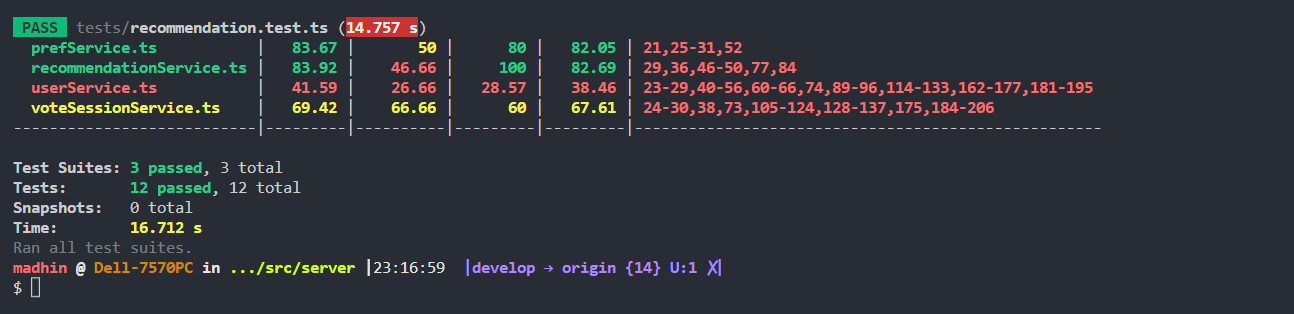
\includegraphics[scale=.4]{Code Coverage Report BE.png}
	\end{adjustwidth}
\end{figure}



\newpage
\section*{Appendix}
\subsection*{Traceability Matrices}
\begin{table}[H]
	\caption{Nonfunctional Requirements Traceability Matrix} \label{TraceMatrix2}
	\begin{tabular}{ll}
		\toprule
		\textbf{Test Number} & \textbf{Requirement} \\
		\midrule
		Look and Feel T 1 & 10.1.1\\
		Look and Feel T 2 & 10.1.2\\
		\midrule
		Usability and Humanity T 1 & 10.2.1\\
		Usability and Humanity T 2 & 10.2.3\\
		\midrule
		Performance T 1 & 10.3.1\\
		Performance T 2 & 10.3.2\\
		Performance T 3 & 10.3.3\\
		Performance T 4 & 10.3.4\\
		Performance T 5 & 10.3.5\\
		Performance T 6 & 10.3.6\\
		\midrule
		Operational and Environmental T 1 & 10.4.3\\
		\midrule
		Maintainability and Support T 1 & 10.5.3\\
		\midrule
		Security T 1 & 10.6.1\\
		Security T 2 & 10.6.2\\
		\bottomrule
	\end{tabular}
\end{table}

\begin{table}[H]
	\caption{Functional Requirements Traceability Matrix} \label{TraceMatrix1}
	\begin{tabular}{ll}
		\toprule
		\textbf{Test Number} & \textbf{Requirement} \\
		\midrule
		UI Auth T 1 & FR 1\\
		API Auth T 1 & FR 1\\
		UI Auth T 2 & FR 1\\
		API Auth T 2 & FR 1\\
		UI Auth T 3 & FR 1\\
		API Auth T 3 & FR 1\\
		UI Auth T 4 & FR 1\\
		API Auth T 4 & FR 1\\
		UI Auth T 5 & FR 3\\
		API Auth T 5 & FR 3\\
		UI Auth T 6 & FR 2\\
		\midrule
		UI PG T 1 & FR 4\\
		API PG T 1 & FR 4\\
		UI PG T 2 & FR 5\\
		API PG T 2 & FR 5\\
		UI PG T 3 & FR 6\\
		API PG T 3 & FR 6\\
		UI PG T 4 & FR 7\\
		API PG T 4 & FR 7\\
		UI PG T 5 & FR 8\\
		API PG T 5 & FR 8\\
		\midrule
		UI R T 1 & FR 9\\
		API R T 1 & FR 9\\
		UI R T 2 & FR 10\\
		API R T 2 & FR 10\\
		UI R T 3 & FR 11\\
		API R T 3 & FR 11\\
		\bottomrule
	\end{tabular}
\end{table}

\begin{description}
	\item M1: Hardware-Hiding Module
	\item M2: Behaviour-Hiding Module
	\begin{itemize}
		\item M3: Native Login Module
		\item M4: Friends Module
		\item M5: Groups Module
		\item M6: Profile Module
	\end{itemize}
	\item M7: Software Decision Module
	\begin{itemize}
		\item M8: Matching Algorithm Module
		\item M9 OAuth Login Module
		\item M10: API Module
	\end{itemize}
\end{description}


\begin{table}[H]
	\caption{Trace Between Modules and Tests}
	\centering
	\begin{tabular}{p{0.2\textwidth} p{0.6\textwidth}}
		\toprule
		\textbf{Module} & \textbf{Tests}\\
		\midrule
		M1 & \\
		M2 & \\
		M3 & UI Auth (T 1-6), API Auth (T 1-6) \\
		M4 & \\
		M5 & UI PG (T 4, 5), API PG (T 4, 5)\\
		M6 & UI PG (T 1-3), API PG (T 1-3)\\
		M7 & \\
		M8 & UI R T 4, API R T 4\\
		M9 & \\
		M10 & UI R (T 1-3), API R (T 1-3)\\
		\bottomrule
	\end{tabular}
	
	\label{TblRT}
\end{table}

\subsection*{Reflection}
Completing the VnV Plan and Report highlighted the effectiveness of the VnV Process. By first completing verification on the system, we got to clearly document the requirements that were thoroughly implemented, the requirements that were missed, and the requirements which were not defined properly and needed to be revisited. Doing so, the SRS and other documents stay fully updated and all the developers stay on the same page regarding the goals of \progname . 

\noindent The other aspect of the VnV Plan were the tests planned for the system, which the report implements. However, a handful of them were misclassified and do not belong in automation testing or duplicates of other tests that could just be a single integration test. While it is important to test each component individually, which unit tests do, having multiple integration tests which do the same thing is a waste of time and resources. By going through the Plan to fill out the Report we found cases which the latter applied, and were subsequently changed to ensure full coverage in our system with developer time allocated appropriately. What's left for verification is to get the CI/CD Pipeline running after the tests have all been merged.

\bibliographystyle{plainnat}

\bibliography{../../refs/References}
\citet{VnVPlan} \\
\citet{SRS} \\
\citet{MG} \\
\citet{MIS} \\

\end{document}